\input{/Users/daniel/github/config/preamble.sty}
\input{/Users/daniel/github/config/thms-eng.sty}
\bibliographystyle{alpha}

\begin{document}

\begin{minipage}{\textwidth}
	\begin{minipage}{1\textwidth}
		\hfill Daniel González Casanova Azuela
		
		{\small Prof. Sergey Galkin\hfill\href{https://github.com/danimalabares/ms}{github.com/danimalabares/ms}}
	\end{minipage}
\end{minipage}\vspace{.2cm}\hrule
\vspace{1em}
{\Huge Minimal Surfaces}

\tableofcontents

\section{Class 1}

\subsection{Intro}

Minimal surfaces started with Lagrange, at 19 years old, more than 250 years old, when he communicated with Euler. Something is minimized. For Lagrange, this was the area functional with respect to euclidean metric \((dx)^2+(dy)^2+(dz)^2\). He was looking for surfaces that \textit{locally} minimize area. He wrote differential equations characterizing this property.

\subsection{Minimizing area of regular surfaces in \(\mathbb{R}^3\)}

\[\begin{tikzcd}
&\mathbb{R}^3=\mathbb{R}^3_{x,y}\perp \mathbb{R}_z\\
\Sigma\arrow[rr,"\pi \circ j:=f_L"]\arrow[ur,"i"]&&\arrow[ul,"\mathbb{R}^2",swap]
\end{tikzcd}\]
The idea is that if \(L \in T_p \Sigma\), then \(f_L\) is locally a diffeorphism around \(p\). {\color{6}dani: So I think that decomposition of \(\mathbb{R}^3\) depends on \(L\).} By inverse function theorem, locally there exists a function \(\varphi(x,y)\) wuch that \(\Sigma=\Gamma_\varphi=\{(x,y,z): z=\varphi(x,y)\}\).

\begin{example}\leavevmode
A sphere is locally seen ass \(z=\sqrt{1-x^2-y^2} \).
\end{example}

\(\Omega \subset \mathbb{R}^2\) some region. Then consider a function that puts the boundary of the region in \(\mathbb{R}^3\) (it's the height function): \(\varphi: \overline{\Omega}\to \mathbb{R}\), \(\varphi|_{\partial\Omega}\). Then minimization of area becomes a PDE on \(\varphi\).

This PDE is historically the first Euler-Lagrange Equation (=equations of motion). Now there's a lot of generalizations of this in classical field theory also.hj n

\section{Class 2}

Lagrange's PDE - nonlinear PDE. From \cite{salsa}:
\[\operatorname{div}\left(\frac{\nabla u}{\sqrt{1+|\nabla u|^2} }\right) =0\]
Laplace equation 
\[\Delta x_i=0\]
and its nonhomogeneous version Poisson equation \[\Delta f=\rho \in \Omega^{2}(\Sigma)\]
\textbf{Rk.} you can think of laplacian on a surface as giving a 2-form by multipliyng by \(\operatorname{Vol}\), this will allow you to integrate. The point is that solution exists  \(\iff\) \([\rho] = 0 \in H^{2}(\Sigma,\mathbb{R})\). If \(\Sigma\) is not compact then there's always a solution. So  \(\Sigma\) compact \(\iff\) \(\int_\Sigma\rho=0\).

So when thinking of Riemann surfaces/complex analysis, if you have \(\Sigma_{(u,v)} \xrightarrow{\varphi}\mathbb{R}^n\) minimal, where \(x_i(u,v)\), then \(x_i\) is a harmonic function wr.t. \(\varphi^* g_{\mathbb{R}^n}\).

\begin{thing4}{Three ways to study minimal surfaces}\leavevmode
\begin{enumerate}
\item \(\sim\) PDE. Colding-Codazzi textbook.
\item Complex analysis/geometry/Riemannsurfaces/practice. Flourished in \(19^{\text{th} }\) century.
\item Geometric measure theory. Very popular these days. Back to Lebesgue (who invented Lebesgue integral when investigating minimal surfaces).
\end{enumerate}
\end{thing4}

Now we comment J. Simons who is the same from Chern-Simons and so many institutions and grants that go by the name Simons.


\begin{thing6}{Result}\leavevmode
In \(\mathbb{R}^3\) there are no closed (compact, without boundary) minimal surfaces.
\end{thing6}

So we look for things with boundary. So from the PDE point of view we look for some boundary condition. This is also called ``plateau problem", which was solved in the 1930's.

\begin{example}\leavevmode
Schwarz minimal surface:
\begin{figure}[H]
	\centering
	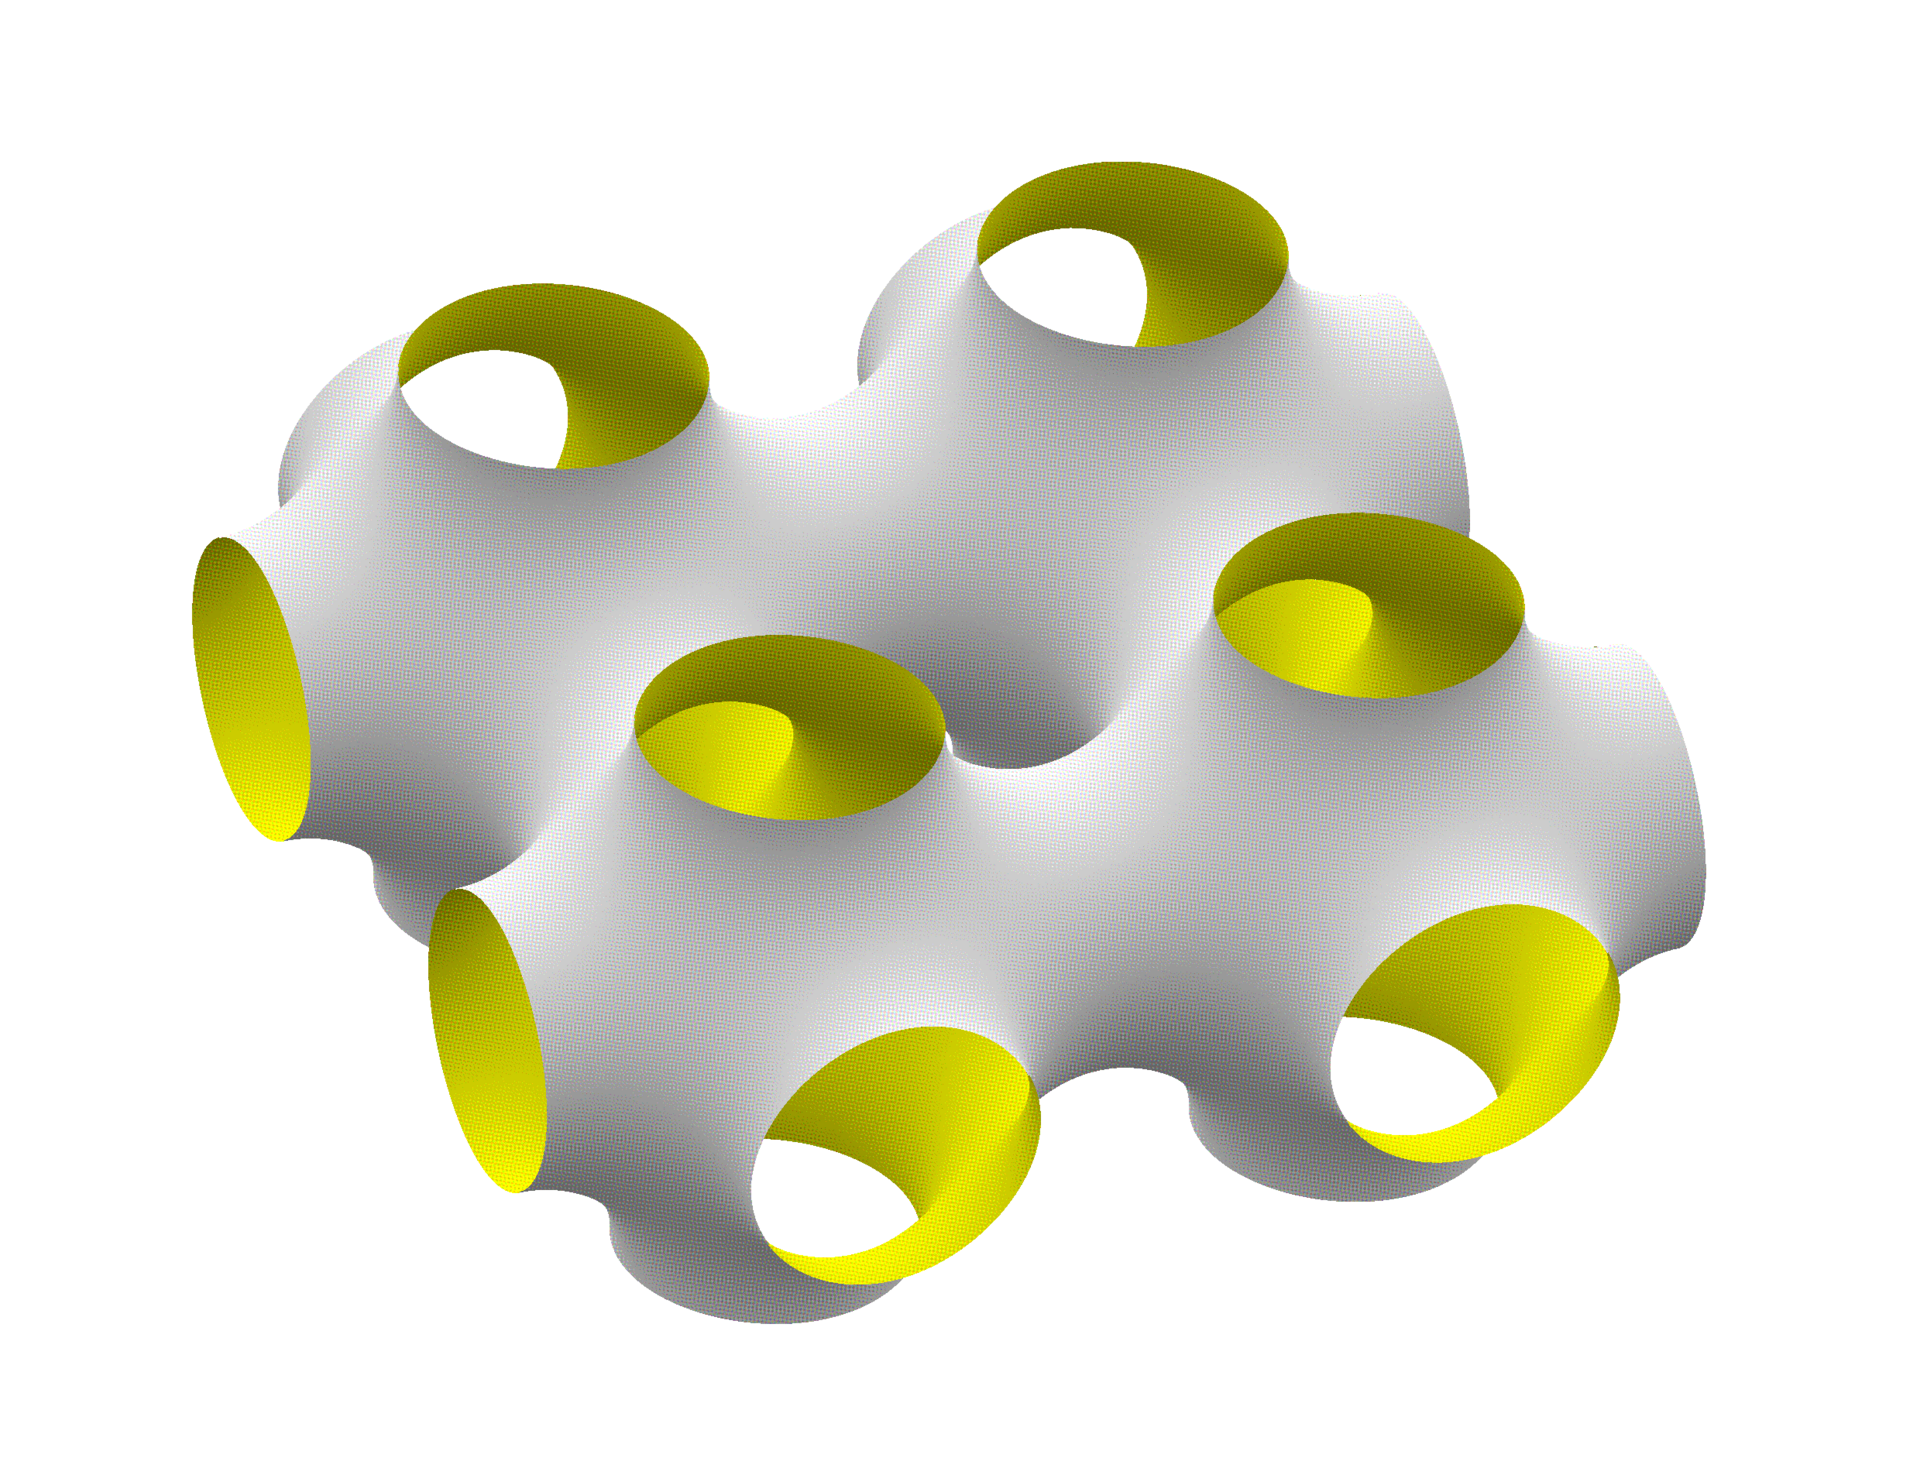
\includegraphics[width=0.5\textwidth]{fig1}
\end{figure}
You can think of this as put inside 3-torus \(\mathbb{T}^3\overset{\operatorname{def}}{=}\mathbb{R}^3/\mathbb{Z}^3\).
\end{example}

\begin{example}\leavevmode
Enneper surface.
\iffalse\begin{figure}[H]
	\centering
	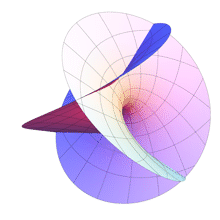
\includegraphics[width=.5\textwidth]{fig2.png}
\end{figure}\fi
\end{example}

*We saw several other examples* In conclusion, minimal surfaces exist and you can see some of them.

\subsection{Basic objects}

Consider
\[M^{(m)}\overset{f}{\hookrightarrow }N^{(n)}=\mathbb{R}^n,\qquad x_1,\ldots,x_n\]
It has a differential
\[T_pM \longrightarrow T_{f(p)}N=\mathbb{R}^n\]
which is a linear map. Now take local coordinates \(D \subset M\), \((u_1,\ldots,u_n)\). Then \(f \) is locally fiven by a functions of \(m\) variables
\begin{align*}
	x_1(u_1,\ldots,u_m)\\
	\vdots \\
	x_n(u_1,\ldots,u_m)
\end{align*}
while \(df_p\) is represented by a \(m\times n\) matrix
\[\left(\frac{\partial x_i}{\partial u_J}\right) ,\qquad  i=1,\ldots,n, j=1,\ldots,m\]
If \(N^{(n)}\cong M^{(m)}\times \mathbb{R}^{n-m}\) and \(f= \operatorname{id}_M \times \varphi\) (so \(M = \Gamma_\varphi\) a graph of \(\varphi\). Then we get a matrix
\[\begin{pmatrix} \operatorname{Id} & * \end{pmatrix} \]
Now look again at \(M \overset{f}{\hookrightarrow }N\). We can pull back the metric of \(N\), which is a symmetric tensor, getting a metric on \(M\). ({\color{6}dani: because \(f\) is immersion=differential is injective).}

So let's try to see how this metric looks like. The pullback metric should of course be something of the kind
\[\sum g_{j j'} du_j du_{j'}\]
now since \(g= \sum (dx_i)^2\) is euclidean metric we get
\[\sum \left(\sum \frac{\partial x^i}{\partial u_j}du_j\right)^2 \]
so that
\[g_{j_1j_2}= \sum \frac{\partial x^i}{\partial u_{j_1}}\frac{\partial x^i}{\partial u_{j_2}}\]
So if this matrix is \(G\) and \(J\) is the jacobian of \(f\) we just get
\[G=J^{\mathbf{T}}J\]

\begin{remark}\leavevmode
We could also just define a metric on \(M\) by putting those coefficient functions and create s symmetric 2-tensor.
\end{remark}
Now consider
\[\bar{g} :=\det(g_{ij})\]
if \(\bar{g}\neq 0 \) then matrix  \((g_{ij})\) is invertible, so it has inverse \((g^{ij})\).

\begin{thing8}{Definition/Proposition}\leavevmode
\(f\) is \textit{\textbf{regular}} in a point \(p\) if any of these equivalent conditions hold:
\begin{enumerate}
\item \(\bar{g}\neq 0\).
\item \(\bar{g}>0\).
\item Vectors \(\left(df_p\right) \left(\frac{\partial }{\partial u_i}\right) \) are linearly independent.
\end{enumerate}
\end{thing8}

\begin{proof}\leavevmode
\end{proof}

\begin{defn}[Cotangent and tangent space]\leavevmode
For a local system of coordinates we can define
\[\Omega_{\mathbb{R}^n}:=\left<dx^{(1)},\ldots,dx^{(n)}\right>\]
as the space generated by the differentials of the coordinate functions. Then we define
\[T_{\mathbb{R}^n}:=\left<\frac{\partial }{\partial x^{(1)}},\ldots,\frac{\partial }{\partial x^{(n)}}\right>\]
as generated by the dual basis of the cotangent basis.
\end{defn}

\subsection{Volume of a submanifold of \(\mathbb{R}^n\)}

Consider \(U,V\) vector spaces and
\[\begin{tikzcd}
	U \arrow[r,"T"]& U \arrow[ r,"\sharp_g"]\arrow[r,"\cong",swap]&  U^{\vee}\arrow[r,"T^*"]&  U^{\vee}
\end{tikzcd}\]
where \(g\) is a metric on \(V\). Then the composition of all this is just the same as the pullback metric on \(U\)! 
\[T^*  \circ \sharp_g \circ T=\sharp_{T^*g}:U \to U^{\vee}\]
Now apply \(\Lambda^{m}\) to get another commutative diagram
\[\begin{tikzcd}
	\Lambda^{m}U \arrow[ r,"\Lambda^{m}T"]\arrow[rrr,bend right,"\bar{g}"]\arrow[d,equals]&\Lambda^{m}V\arrow[r,"\Lambda^{m}\sharp g"]&\Lambda^{m}V^{\vee}\arrow[ r,"\Lambda^{m}T^{\vee}"]&  \Lambda^{m}U^{\vee}\arrow[d,equals]\\
	\mathbb{R}& & & \mathbb{R}
\end{tikzcd}\]
and then the composition here gives us
\[\bar{g}=\sum_{1\leq  j_1\leq \ldots \leq j_m \leq n}\left(\det\left(\frac{\partial x^{j_k}}{\partial u_i}\right) \right) ^2\]

Let \(v_1,\ldots,v_n\) be a basis of \(U\) and \(e_1,\ldots,e_n\) another basis. Let \(V\) be a matrix that takes one basis to another. Then
\[G=V^{\mathbf{T}}V\]
\[\implies \det G= \det(V)^2\implies \bar{g}(p)=\operatorname{Vol}_M\Big((df)_p\left(\frac{\partial }{\partial u_1}\right),\ldots,(df)_p\left(\frac{\partial }{\partial u_n}\right) \Big)^2 \]

\begin{defn}[Volume of \(M \overset{f}{\hookrightarrow }\mathbb{R}^n\)]\leavevmode
 \[\operatorname{Vol}M=\int_M\sqrt{\det g}du_1\ldots du_m \]
\end{defn}

Which takes us to the problem of volume minimzation.

Then followed some computation of the minors of
\[\begin{pmatrix} 1&0&z_x\\0&1&z_y \end{pmatrix}\ldots \]

\begin{thing6}{Extra, we discussed this at some time}\leavevmode
That \textit{\textbf{hypersurface}} is a thing locally defined by \textit{one} function.
\end{thing6}

\section{Class 3}

\subsection{Isothermic coordinates}

A \textit{\textbf{Weyl transformation}} is a map of metrics
\[g \mapsto  e^kg\]
where we use exponent just to mean an invertible positive number. \(k\) is a real function.

\begin{upshot}\leavevmode
That a metric on a surface induces a complex structure given by anticlockwise 90-degree rotation. And the interesting part is that two conformal metrics induce the same conformal structure, and the map that relates these metric is the Weyl transform.
\end{upshot}

\begin{thing8}{Example: euclidean coordinates}\leavevmode
Euclidean metric is \((du)^2+(dv)^2\). Letting \(dz:=du+idv\) and \(d\bar{z}:=du-i dv\) we get
\[(du)^2+(dv)^2=(dz)\cdot(d\bar{z})\]
Now take other coordinates \(w\), \(w=F(z)\).  You'll get
\[dw\cdot d \bar{w}=\underbrace{|F^i(z)|^2}_{e^k}dz\cdot d\bar{z}=e^k((du)^2+(dv)^2)\]
And the matrix is
\[\begin{pmatrix}e^k&0\\ 0&e^k\end{pmatrix}\]

\textbf{Conclusion:} conformal class of metric is the same as complex structure.
\end{thing8}

\begin{defn}\leavevmode
\textit{\textbf{Isothermic coordinates}} are local coordinates \((u,v)\) such that \(g_{11}=g_{22}\) and \(g_{12}=0\). So,  \textbf{scalar} multiple of euclidean metric.
\end{defn}


\begin{claim}\leavevmode
Any Riemannian surface \((\Sigma,g)\) has local isothermic coordinates. (In fact, for every power series we get another isothermic coordinates. There is a group action of the \textit{\textbf{local biholomorphisms}}. In higher dimension this is only finite dimensional, generated by inversions (this is a group, like inversion about circle in \(\mathbb{C}\)) and isometries (i.e. \(\operatorname{Isom}(\mathbb{R}^n) \supset\mathsf{O}(n),\mathbb{R}^n\)). So conclusion: in dimension 2 it has to do with complex analysis and in higher dimension it's just different.)
\end{claim}

\begin{thing7}{We have learnt}\leavevmode
that there are some thing of complex analysis like maximum principle and probably also Schwarz principle that generalize to higher dimension, but not everything.
\end{thing7}

\begin{remark}\leavevmode
Recall that conformal maps are either holomorphic or antiholomorphic.
\end{remark}

\subsection{Gauss map}

\subsubsection{Grassman and normal bundles}

Recall what is grassmanian \(\operatorname{Gr}(m,n)\) with \(m<n\), the variety of \(m\)-dimensional vector subspaces of an \(n\)-dimensional vector space \(V\), and Plucker embedding \(\operatorname{Gr}(m,n)\hookrightarrow \mathbb{P}\Lambda^{m}V\).


\begin{defn}\leavevmode
\(V\) has \textit{\textbf{vectors}}. \(V^\vee\) has \textit{\textbf{covectors}}.  \(\Lambda^{2}V\) has \textit{\textbf{bivectors}}.  \(\Lambda^{3}V\) \textit{\textbf{trivectors}}.  \textit{\textbf{Polyvectors}}. For bundles:  \(\Lambda^{2}T_M\) \textit{\textbf{bivector fields}}.  \(\Lambda^{m}T_M\) \textit{\textbf{polyvector (or multivector) fields}}, they are dual to  \(\Omega^{m}=\Lambda^{m}\Omega\), differential \(m\)-forms.
\end{defn}
For a subspace \(U \subset V\) we get corresponding \(\underbrace{\Lambda^{m}U }_{\substack{\text{1-dim case}  \\ \cong\mathbb{R}}}\xrightarrow{\Lambda^{m}j}\Lambda^{m}V\)
and corresponidingly
\[\underbrace{\mathbb{P}\Lambda^{m}U}_{\substack{\text{1 dim}  \\ =pt}}\xrightarrow{\mathbb{P}(\Lambda^{m}j)}\mathbb{P}\Lambda^{m}U\]

Next. If \(V=\mathbb{R}^n\) is equipped with a metric \(g\) you have for two orthonormal bases
\[e_1 \wedge \ldots \wedge e_m=\det C f_1\wedge \ldots \wedge f_m\]
For a map \(f_i=C_i^j e_j\). If they are orthonormal you get \(\det C=\pm 1\) and of you orient it all you get \(\det C=1\).

Correspondingly define the space of \textit{oriented} vector subspaces of euclidean space by \(\operatorname{Gr}^+(m,\mathbb{R}^n)\).
For a basis \(U=\left<u_1,\ldots,u_m\right>\), we get a basis \(\Lambda^{m}U=\left<u_1\wedge u_2\wedge\ldots \wedge u_m\right>\).

\begin{example}\leavevmode
\begin{itemize}
\item \(\operatorname{Gr}(1,2)=\) circle.
\item \(\operatorname{Gr}^+(1,2)\) space of rays.
\item \(\operatorname{Gr}^+(1,\mathbb{R}^n)=S^{n-1}\).
\item \(\operatorname{Gr}(1,\mathbb{R}^n)=\mathbb{R}P^{n-1}\).
\end{itemize}
\end{example}

Now do
\[\begin{tikzcd}0\arrow[r]&U^{(m)}\arrow[r]&V^{(n)}\arrow[r]&Q^{(n-m)}\arrow[r]&0\end{tikzcd}\]
dualize
\[\begin{tikzcd}0\arrow[r]&Q^\vee\arrow[r]&V^\vee\arrow[r]&U^\vee\arrow[r]&0\end{tikzcd}\]
So you automatically get isomorphisms
\[\operatorname{Gr}(m,V)=\operatorname{Gr}(V,n-m)=\operatorname{Gr}(n-m,V^\vee)=\operatorname{Gr}(V^\vee,m)\]
Now apply \(\Lambda\):
\begin{exercise}\leavevmode
\(\Lambda^{n}V \cong \Lambda^{m}U \otimes \Lambda^{n-m}Q\)
\end{exercise}

\begin{proof}[Attempt of solution]\leavevmode
The exact sequence above gives \(V=U \oplus  Q\), so that \(\Lambda^{n}V=\Lambda^{n}(U \oplus  Q)\).  So I think well \(\Lambda^{n}V\) is just tensor of \(V\) \(n\) times quotiented by the antisymmetry relation \(x \otimes x=0\). And that's close but not exactly…
%\[V^{\otimes n}=(U \oplus  Q)^{\otimes n}\neq \bigoplus_{k}\underbrace{\binom{n}{k}}_{\substack{\text{tensor}  \\ \text{not} \\\text{commut.} }}U^{\otimes n-k} \otimes Q^{\otimes k}\overset{\text{want}{\rightsquigarrow } U^{\otimes m}\otimes Q^{\otimes (n-m)}\]

\end{proof}

\begin{example}\leavevmode
\(\operatorname{Gr}^+(2,3)=S^2=\) conic \(\subset\mathbb{C}P^{2}\), more exactly \(\{x^2+y^2+z^2=0\}\).
\end{example}

\begin{exercise}\leavevmode
\(\operatorname{Gr}^+(2,\mathbb{R}^n)\cong Q^{n-2}\subset \mathbb{C}P^{n-1}\) of the form \(\left\{\sum_{i=1}^n z_i^2=0\right\}\)
\end{exercise}

\begin{proof}[Solution]\leavevmode
When is a complex subspace of a complex vector space expressed with real coordinates?

Here's the general statement. For any \(U_\mathbb{C} \subset V_\mathbb{C}\), the following are equivalent
\begin{itemize}
\item There exists \(U_{\mathbb{R}} \subset V_\mathbb{R}\) such that \(U_\mathbb{C} = U_\mathbb{R} \otimes \mathbb{C}\) (equations are real)
\item \(\overline{U_\mathbb{C}}=U_\mathbb{C}\) where bar denotes all the complex conjugate vectors inside the space, i.e. \(\text{bar}:V_\mathbb{C} \to V_\mathbb{C} \), \((z_1,\ldots,z_n) \mapsto (\overline{z_1},\ldots,\overline{z_n}\). In conclusion, \(\sum a_i\cdot z_i=0 \iff \sum \overline{a_{\bar{i}}}\overline{z_{\bar{i}}}=0\).
\item \(\overline{\Lambda^{m}U_\mathbb{C}}=\Lambda^{m}U_\mathbb{C} \in \Lambda^{m}V_\mathbb{C}\).
\item \(\exists  \pi \in \Lambda^{m}V_\mathbb{C}\) s.t. \(\Lambda^{m}U = \pi \otimes_\mathbb{R} \mathbb{C}\).
\end{itemize}
the point is that these points have \textbf{real Plücker coordinates}.

``for complex isotropic vector construct a real bivector (the line is the same)" And every multiple of this vector gives you the same line. So you can projectivize. So for any point in the projectivized quadric we get a line. And also we can conjugate and get the same line. So that's from quadric to grasmannian. Choice of orientation is a choice of the two points.
\end{proof}

\begin{remark}[dani]\leavevmode
Lo que yo entendí: te pegas la métrica euclidiana real en el subespacio. Es una forma quadráitca. Como es positiva no degenerada no hay zeros. Pero complejificas y obtienes que sí hay zeros, de hecho, tienen que ser dos zeros. Esos zeros creo que son zeros en el plano. Pero orientas, entonces hay uno nomás. E é isso, esse aí é um mapa bijetivo entre a quadrica e a grasmanniana orientada.
\end{remark}

\begin{remark}\leavevmode
And this has all to do with Weierstrass representation.
\end{remark}

\subsubsection{Gauss map}
Consider 
\[M^{(m)}\xrightarrow{f}N^{(2)}\]
and do
\[\mathbb{R}^m \cong T_p^m M \xrightarrow{d_pf}T_{f(p)}N \cong \mathbb{R}^n\]
so for every regular (=rank is \(m\)=the map is an embedding=the thing is a subvariety) \(p\) you get a point in grassmanian
\[\operatorname{Gr}(m,T_{f(p)}N)\]
Consider \(f^*T_N\) which is a vector bundle over \(M\), then we can consider
\[(df):T^{(m)}_M \overset{\text{by regularity,} }{\hookrightarrow } f^*T^{(n)}_N \to \underbrace{f^*(T_N / df(T_M))^{(n-m)}}_{\text{\textit{\textbf{normal bundle}}} }\]
and then consider the \textit{\textbf{Grassmanization}} of \(f^*T_N\), which is a bundle
\[\begin{tikzcd}
\operatorname{Gr}(m,f^*T_N)\arrow[d]\\
M
\end{tikzcd}\]

Now consider sections of this thing.

\begin{thing7}{Important observation}[Gauss map definition]\leavevmode
 Given a trivialization of \(f^*T_N\), a section of the thing becomes just a map
 \[M \to \operatorname{Gr}(m,n)\]
 (Because a section of a trivial bundle is just a map to the fiber.) 
\end{thing7}

Now fix \(N:= \mathbb{R}^n\) and put a connection, the Levi-Civita connection. Actually now better take the oriented Grassmanian for the whole bussiness. And we have the map
\[M \to \operatorname{Gr}^+(m,n)\]
which is a map that to every point associates its tangent space. And it is called the \textit{\textbf{Gauss map}}.

Recall that
\begin{claim}\leavevmode
A surface is minimal \(\iff\) Gauss map is conformal (anti-holomorphic).
\end{claim}

Put a surface in \(\mathbb{R}^3\). Basis for tangent space is
\[(x_u,y_u,z_u), (x_v,y_v,z_v)\]
So basis for projectivization is
\[(y_uz_u-y_vz_u, x_uz_v-x_vz_u,x_uy_v,x_vy_u)\]
and in general, when you get
\begin{align*}
\Sigma&\to \mathbb{R}^n\\
\frac{\partial x}{\partial u}, \frac{\partial x}{\partial v} &\rightsquigarrow \frac{\partial x}{\partial u}\wedge \frac{\partial x}{\partial v}
\end{align*}
\begin{thing8}{Lesson}\leavevmode
Plücker coordinates of oriented Grassmanian are the same as coordinates of normal bundle!
\end{thing8}
But also notice that you can write
\[\{x^i,x^j\}_{du \wedge dv}\]
And the point of all this is that 

\begin{claim}\leavevmode
Minimal surfaces are equivalently defined as the ciritical points of the \textit{\textbf{Schild action}} 
\[\int \left(\sum_{i<j}\{x_i,x_j\}^2\right)\omega\]

\end{claim}
Now put a curve \(I \subset \Sigma \to \mathbb{R}^n\)… [what was the curve for…?]

\begin{thing7}{Hint}\leavevmode
From 1 to 2 you ``vary" the volume and look for critical points.
\end{thing7}

\begin{thing6}{Important exercise}\leavevmode
If \(x=u,y=v\) and \(z=\varphi(u,v)\), you get two derivatives
\[\partial_u \to (1,0,\varphi_u)\qquad \partial_v \to (0,1,\varphi_v)\]
Notice that
\[df[\partial_u]=\partial_x+\varphi_u\cdot \partial_z\]
And now
\[\partial_u \wedge \partial_v = \partial_u \wedge \partial_y- \varphi_v\partial_x \wedge\partial_z-\varphi_v \partial_y \wedge \partial_z\]
Then you have proportionality
\[N \sim (-\varphi_u,-\varphi_v,1):=\tilde{N}\]
So
\[\|\tilde{N}\|^2=\varphi_u^2+\varphi_v^2+1=g\]
\[N=\frac{\tilde{N}}{\sqrt{g} }\]
So \textit{\textbf{Gauss map for non-parametric surface}} is 
\[G:(u,v) \longrightarrow\left(\frac{-\varphi_u}{\sqrt{1+\varphi^2_u+\varphi^2_v} },\frac{-\varphi_v}{\sqrt{1-\varphi^2_u+\varphi^2_v} },\frac{1}{\sqrt{1-\varphi_u^2+\varphi_v^2} }\right) \]
(and you can just write \(\sqrt{1+\varphi_u^2+\varphi_v^2} =\sqrt{g} \) but Ok). Similarly…
\end{thing6}

\subsubsection{Second fundmental form}

And differentiate! At every point we get
\[d_pG:T_pM \to T_{G(p)}\operatorname{Gr}(m,n)=\operatorname{Hom}(T_pM,N )\]
(where \(N\) is the normal bundle). So globally
\[dG \in \operatorname{Hom}(T_pM,\operatorname{Hom}(T_pM, N))\]
So it's a map aa
\(T_pM \times T_pM \to N\) 
But \(N\) is trivialized! So you can think of  \textit{numbers}. So it's a form.

\begin{claim}[Exercise]\leavevmode
That map is symmetric.
\end{claim}
So you can define it to be the \textit{\textbf{second fundamental form}}.


\begin{thing8}{Notations}\leavevmode
\begin{itemize}
\item I fundamental form \(\rightsquigarrow \) \(g_{ij}\).
\item  II fundamental form \(\rightsquigarrow \) \(B_{ij}\) for a vector in the normal bundle, and \(b_{ij}\) when you are in \(\mathbb{R}^3\) and you have trivialized it to get numbers
\end{itemize}
\end{thing8}

\begin{claim}\leavevmode
\[B_{ij}=\left(\frac{\partial^2 \vec{x}}{\partial u_i\partial u_j}\right)^N \]
where exponent \(N\) means projection to the normal bundle which can mean algebraic projection when you think of a quotient bundle or orthogonal projection when you think geometric.
\end{claim}

\subsection{Reminder: variational approach}

\begin{thing6}{Reminder of the end of last lecture}[Variation of the tangent direction]\leavevmode
	\begin{align*}V'(t=0)[\underbrace{\delta \varphi}_{:=w}]&= \int_{\Sigma}\frac{z_x\cdot w_x+z_y\cdot w_y}{\sqrt{g} }dudv\\
		&=\int \left<\delta \varphi,\text{something} \right>\frac{\sqrt{g} dudv}{\text{volume form} }
	\end{align*}
where \(\delta \varphi\) is a section of \(f^* T_{\mathbb{R}^n}=df(T_M) \oplus^\perp N\). And \textbf{something} is a unique thing that exists making the equality hold. This is a possible definition of \textit{\textbf{mean curvature vector}} \(\vec{H} \in N\).

And you can also write
\[\int dv \wedge \left(\frac{z_u}{\sqrt{g} \cdot w_u du}\right) = \int dv \wedge \left(\frac{z_u}{\sqrt{g} }dw\right) \]
where \(dw=w_u du+\ldots+dv\). And now we want to integrate by parts to get
\[=-\int w \cdot \partial\left(\frac{z_u}{v_g}dv\right) \]
So the integral above (with the \textbf{something} inside) becomes
\begin{align*}
\int_{\Sigma}\frac{z_x\cdot w_x+z_y\cdot w_y}{\sqrt{g} }dudv&=-\int \left(\partial_u \frac{z_u}{\sqrt{g}}+\partial_v \frac{z_v}{\sqrt{g}}  \right)\cdot w du dv
\end{align*}
so if that is zero for all \(w\), then the thing in parenthesis must be zero by nondegeneracy of metric.
\end{thing6}

Right so what is the \textit{\textbf{first variation of volume}}? It's
\[V'|_{t=0}=-\int_\Sigma(\sqrt{g} du) \left<H,W\right>\]
And it has all to do with the expression \(\Sigma g^{ij}B_{ij}\).

\section{Class 4}

\section{Class 5}

\subsection{Classical Field theory: fields, lagrangian and action}

\begin{enumerate}
\item \textit{\textbf{Field}}: the map \(\varphi:\Sigma \to X\).
\item \textit{\textbf{Action}}: \(S[\varphi]=\int_\Sigma \underbrace{\mathcal{L}[\varphi]d \operatorname{Vol}_\Sigma}_{\text{Lagrangian density} }\).

	You give me a field, I give you a top-form, i.e. something you can integrate in \(\Sigma\). That's the idea of the Lagrangian. So \(\mathcal{L}(\varphi)\) is a ``rule" to produce densities from fields. \(\mathcal{L}[\varphi]\) is a local operator. \(\mathcal{L}[\varphi]\) depends on the fields and their derivatives. Classical version is \(\mathcal{L}=E - U\) i.e. kinetic \(-\) potential energy.
\item \textit{\textbf{Equation of motion (EOM):}} are the critical points of \(S\)
\end{enumerate}

\subsection{Area functional aka Nambu-Goto action}

\[S_{\operatorname{ NG}}[\varphi]=\int_{\Sigma}d\operatorname{Vol}_{\varphi^*g}\]
where \(d\operatorname{Vol}_G=\sqrt{- \det G_{ij}}\) where \(\varphi: \Sigma \to X\) and \(X\) might have lorenzian metric, so that's why there's  sign.

\subsection{Polyakov action}

It's \textbf{a thing that depends both on \(h\) and \(\varphi\)}: 
\[S_{\text{pol} }[\varphi;h]=\int_{\Sigma}d\operatorname{Vol}_h \|d\varphi\|_g^2\]
where \(\|d \varphi\|^2\) might as well be explained in the context of:

\subsection{Dirichlet energy/energy functional}

\[\operatorname{tr}\left(\begin{tikzcd}T_p\Sigma \arrow[r,"df"]&  T_{f(p)}X\arrow[d,"\sharp_g"]\\T_p^\vee \Sigma \arrow[u,"(\sharp_h)^{-1}"]&  T_{f(p)}X \arrow[l,"(df)^\vee"]\end{tikzcd}\right) \]
which gives
\[\frac{\partial X^\mu}{\partial u_i}g_{\mu\nu}(\varphi(u))\frac{\partial X^\nu}{\partial u_j}h^{ij}\]
So you give me a map, I give you a number. $\mathsf{OK}$ but definition of of \textit{\textbf{Dirichlet energy/energy functional}} it's actually the same thing as Polyakov action but \textbf{\(h\) is fixed}:
\[E_{h}(\varphi)=\int_{\Sigma}d\operatorname{Vol}_h \|d\varphi\|_g^2\]

\begin{thing8}{Important example}\leavevmode
If we take usual euclidean metrics we get usual laplacian operator and usual harmonic functions.
\end{thing8}

\begin{thing8}{Nice example}\leavevmode
If you had a line instead of a surface, i.e. \(\Sigma=\mathbb{R}\) then you'd get that the it is a geodesic (in \(X\)) iff… the map is harmonic!
\end{thing8}

\begin{upshot}\leavevmode
That's what's going on: harmonicity characterizes minimizing these functionals. So minimal surfaces, geodesics, appear along with geodesics.
\end{upshot}

\subsection{Harmonic function}

\begin{defn}\leavevmode
A map \(\varphi:(\Sigma,h) \to (X,g)\) is called \textit{\textbf{\((h,g)\)-harmonic}} if it is a critical point of the energy functional
\end{defn}

So in terms of Polyakov action you have some equations of motion (=critical points of P. action):
\begin{enumerate}
\item \(\frac{ \delta S}{\delta \varphi}=0\) i.e. \(\varphi\) is \(h\)-harmonic.
\item \(\frac{\delta S}{\delta h}=0\) some other thing we'll study up front.
\end{enumerate}

\subsection{Symmetries of Dirichlet energy}

Weil transformations (conformal transformations= take the metric and multiply by a function) preserve Dirichlet energy. Which is a complex structure (the conformal class of the metric). We mean--- \(E\) depends on the complex structure of \(\Sigma\).

\subsection{Feynman quantization}

\[Z(\hslash)=\int_{\text{Fields} }e^{\frac{i S[\varphi]}{\hslash}}\mathcal{D}\varphi\]

\subsection{The other critical point of Polyakov}

Recall that Polyakov depends both on \(h\) and \(\varphi\). So there must be some interpretation of
\[\frac{\delta S}{\delta h}=0.\]
First we need to differentiate determinant. See \href{https://en.wikipedia.org/wiki/Adjugate_matrix#Jacobi's_formula}{wiki}, cofactor matrix appears. So the inverse matrix appears.
\[\text{*more computations*} \]
\begin{quotation}
	``So 2nd EOM says that \(h \) and \(G\) (I fundamental form of \(\varphi^*g\)) lie in the same conformal class (and also shows the exact solution)"
\end{quotation}
So they give the same complex structure. And it goes back to Nambu-Goto action---we get rid of the \(h\).

\subsection{Mean curvature vector (again)}

\(\vec{H}(u)\) is a normal vector such that
\begin{enumerate}
\item \[\delta S_{\operatorname{ NG}}=\int \delta \vec{X}\cdot \vec{H}\operatorname{Vol}g\]
for any variation \(\delta \vec{X}\).
\item \(\vec{H}=\Delta \vec{X}\).
\item \(\vec{H} =B_{ij}G^{ij}\)
	where
	\[B_{ij}=\left(\frac{\partial^2 \vec{X}}{\partial u_i\partial u_j}\right) \text{\(\leftsquigarrow \) II fundamental form} \]
	so the projection to normal space.
\item \(\vec{H}=\operatorname{tr}(S)\) (mean curvature is the trace of shape operator.) So \textit{\textbf{shape operator}} is
	 \[S:=\sharp^{-1}_G \circ \sharp_B,\]
	an operator on  \(T \Sigma\) valued in \(f^*N\).
\end{enumerate}

\begin{exercise}\leavevmode
\begin{enumerate}
\item Prove \(1 \iff 2 \iff 3\). \textbf{Hint.}  You write the variation formula and integrate by parts and that's it.
\item Write them down in case \(n=3\). \(\varphi\) grpo off \(u,v \to (u,v,f(u,v))\), \(G_{ij}\), \(G^{ij}\), \(B^{ij}\).
\end{enumerate}\end{exercise}

\begin{defn}\leavevmode
\textit{\textbf{Third fundamental form}} is…
\end{defn}

\section{Class ?}

\subsection{Vier bein}

If you happen to read the paper by Shild (?) (or is it ``The relativistic string" you may find the concept of \textit{\textbf{vier bein}} which is equivalently a choice of local orthonormal base of a vector bundle and a filtration \(F^1\subset F^2 \subset F^3 \subset\ldots F^n = E\). (So you just choose the first \(i\) of the orthonormal sections to produce \(F^i\).) What's nice about this is that you allow the sections to be nonconmutative, unlike the \(\partial_i\) which satisfy \([\partial_i,\partial_j]=\delta_{ij}\).

\subsection{Schild action}

\begin{enumerate}
	\item Length: \(\delta\left(m \int_{u^*}^{u^{* *}}[(\dot x)^2]^{\frac{1}{2}}du\right) \)
	\item Energy: \(\delta\left(_{u^*}^{u^{* *}}\frac{1}{2}(\dot x)^2\right) \)
\end{enumerate}

\begin{question}\leavevmode
\begin{enumerate}
\item why variation is defined in terms of velocity
	why delta s2 = only the mid term in the xapsion
\end{enumerate}
\end{question}

\begin{remark}\leavevmode
First variation formula shows: critical point of length functional \(\implies\) geodesic  \(\dot \dot x=0\)
\end{remark}

\begin{defn}\leavevmode
\textit{\textbf{Mean curvature flow}} is such that its derivative is \(\vec{H}\).
\end{defn}

\section{Class}

\begin{claim}\leavevmode
Locally any harmonic function
\end{claim}

\section{Class}

\begin{enumerate}
\item Two definitions of hodge star.
\item Second definition gives an isomorphism \(\det V\otimes \Lambda^{k}\cong \Lambda^{n-k}V\) 
\item \(d^*=* \circ d \circ *\)
\begin{exercise}\leavevmode
Notice that in the case of \(n=2k\) we have that \(*_g:\Omega^{k}(V)\to \Omega^{k}(V)\). For \(n=2\), \(k=1\), show that \(*_g=J_g\), where \(J_g\) is the almost complex structure defined by \(g\) (discussed in earlier sessions).
\end{exercise}
\item Laplace operator on Riemannian manifolds: \(\Delta^g:=[d,d^*]=d d^*-d^* d=d * d *- * d * d.\)
\item \textit{\textbf{Harmonic \(k\)-forms}}: \(\ker \Delta^g:\Omega^{k}(M)\to \Omega^{k}(M)\).
\item Notice that \(\Delta^g=\underbrace{* d *}_{\operatorname{div}}\underbrace{d}_{\operatorname{grad}}\) matches the other definition for laplacian in riemannian manifolds.
	\item \textbf{Thm (E. Hopf).} For any \((M,g)\), harmonic functions satisfy \textit{\textbf{maximum principle}}. That is, any harmonic function \(f:U \to \mathbb{R}\) for \(U\) connected and open, if \(\exists p \in U\) that is a local maximum or local minimum, then \(f\) is constant on \(U\). (So if \(f\) was nonconstant the point should be in the boundary somehow.)
	\item Another definition of laplacian: \(\Delta^g=\sum(\xi_k)^2+\nabla_{\xi_k}\xi_k\)for an orthonormal frame \(\xi_k\), where \(\xi_k^2\) means apply \(\xi\) as a differential operator twice. So this is a second order differential operator. So if you are euclidean the \(\nabla\) part vanishes (so maybe think of Christoffel symbols) and you are left with the other part, which is usual laplacian.

\item \textbf{Prop.} On euclidean space, \(\Delta=\sum\partial_i^2\).
\item \textbf{Prop (mean value).} \(\Delta f=0 \iff \forall  B (P,R)\) ball,
	\[f(P)=\frac{1}{\operatorname{Vol} B}\int f(Q) \operatorname{Vol}_g\]
	which is the mean value of \(f\) in \(B\). (Comment: you can derive mean value property from Cauchy integral formula.)
\item Another remark about mean value property: holds in general for manifolds. For surface case it's easier because we have isothermal coordinates.
\item Recall that for \(X:\Sigma \to \mathbb{R}^n\) we have a laplacian \(\Delta_g \vec{X}=(\Delta X^1,\ldots,\Delta X^n)\) because vector fields on \(\mathbb{R}^n\) are vectors in \(\mathbb{R}^n\). So we showed at some point that \(\Delta_g \vec{X}=\vec{H}\).
\item Then a remark on isothermal coordinates: basic vectors are orthogonal and of the same size.
\item Now consider
	\[\phi^\alpha(u,v)=\frac{\partial X^\alpha}{\partial u}-i \frac{\partial X^\alpha}{\partial v}\]
(I think \(\phi\) is a map \(\mathbb{R}^2 \to \mathbb{R}^2=\mathbb{C}\).) So \textbf{Claim.} \(X^\alpha\) is harmonic \(\iff\) \(\phi^\alpha\) is holomorphic.

Recall from complex analysis that \(\Delta f=0 \iff \partial_z f\) is holomorphic. So choose for \(f\) one of the component functions of the map \(X\).

\item So notice: when you have a minimal surface you have \(X\) is harmonic so \(\phi^\alpha\) will be holomorphic for all \(\alpha\). Then, in conformal coordinates (cf. isothermal coordinates above), we get
	\[\operatorname{Re}\vec{\phi} \perp \operatorname{Im}\vec{\phi},\qquad |\operatorname{Re}\vec{\phi}|=|\operatorname{Im}\vec{\phi}|.\]
\item  Now the other direction: if you get the data from the last equation, can you construct a minimal surface? So first notice that
	\[d X^\alpha=\frac{\partial X^\alpha}{\partial u}du+\frac{\partial X^\alpha}{\partial v}dv.\]
	Then some computation followed and we conclude that
	\[X^\alpha(p)=\operatorname{Re}\int_{p_0}^pQ(z)dz, \qquad z=u+iv\]
And then
\begin{claim}\leavevmode
If \(Q^\alpha(z)dz\) are holomorphic differentials on \((\Sigma,J)\) + connection, then the last equation gives a minimal surface in \(\mathbb{R}^n\). And then some more computations and we conlcude that
\[\text{conformal coordinates} \iff \sum \phi_k(z)^2=0 \]
So you have a collection of holomorphic functions that their sum of squares equals zero.

\end{claim}
\item \textit{\textbf{Weierstrass data}}:
	\begin{enumerate}
	\item A complex structure \(J\) on \(\Sigma\).
	\item \(\alpha_1,\ldots,\alpha_n \in \Gamma(\Sigma_J,\omega_\Sigma)\) such that
		\[\sum_{k=1}^n(\alpha_k)^2=0 \in \Gamma(\Sigma_J,\omega_\Sigma^{\otimes 2})\]
	\item \(\forall \gamma \in H_1(\Sigma,\mathbb{R})\) s.t. \(\forall k=1,\ldots,n\),
		\[\operatorname{Re} \int_\gamma \alpha_k=0\]
		``Global conditions on periods"
	\end{enumerate}
\begin{claim}\leavevmode
Weierstrass data \(\iff\) Minimal surfaces with
\[\vec{X}(p)=\operatorname{Re}\int_{p_0}^p \vec{\alpha}.\]
\end{claim}
\end{enumerate}
\subsection{Maximum principle}

\begin{thing7}{Maximum principle}[E. Hopf]\leavevmode
\textbf{(Class statement.)} For any \((M,g)\), harmonic functions satisfy \textit{\textbf{maximum principle}}: any harmonic function \(f:U \to \mathbb{R}\) for \(U\) connected and open, if \(\exists p \in U\) that is a local maximum or local minimum, then \(f\) is constant on \(U\).

We shall show Do Carmo's version that \(f\) \textit{\textbf{subharmonic}}, i.e. \(\Delta f\geq 0\), on \(M\) compact connected \(\implies\) \(f\) constant. (This is Exercise 12, Chapter III, \cite{doc}, and all steps are just other exercises from the chapter of Geodesics :))
\end{thing7}

\begin{proof}\leavevmode
\begin{enumerate}[label=\textbf{Step \arabic*}]
	\item \textbf{(Exercise 7, Chapter III of  \cite{doc}.)} Make sure you can pick a \textit{\textbf{referencial geodésico}} about every point of \(M\). This is an orthonormal frame \(\{E_i\} \subset \mathfrak{X}(U)\), where \(p \in U\) such that \(\Big(\nabla_{E_i}E_j\Big)_p=0\). This frame can be obtained by taking geodesic coordinates at the point, an orthonormal base \(\{e_i\}\) of \(T_pM\), and taking parallel transport of the vectors \(e_i\) along radial geodesics emanating from \(p\). This immediately ensures that \(E_i\) is orthonormal since parallel transport preserves angles.

		To check that Christoffel symbols vanish at \(p\) we do as follows. (This is actually a basic fact about geodesic coordinates, see \cite{ler} Prop. 5.24.) Take a random vector \(v \in T_pM\) and its geodesic \(\gamma_v(t)=\operatorname{exp}_p(tv)\). I drop the subindex \(v\) for the next computations for the next computations. Then (this is Florit way of using covariant derivative along a curve; it's the \textit{\textbf{pullback}} or \textit{\textbf{induced connection}} \(\nabla^{\gamma}\)):
		\begin{align*}
			0&=\nabla_{\frac{d}{dt}}^{\gamma}\gamma'=\nabla^{\gamma}_{\frac{d}{dt}}v^i(E_i\circ \gamma)
		\end{align*}
		where the \(v=(v^1,\ldots,v^n)\). Indeed: this is very silly but, since the coordinate chart of geodesic coordinates is \(\operatorname{exp}_p^{-1}\), the coordinate representation of \(\gamma\) in this chart is as simple as
	\[\hat{\gamma}(t)=(\underbrace{\varphi}_{\text{chart}} \circ \gamma)(t)=\operatorname{exp}_p^{-1} \operatorname{exp}_p(tv)=tv.\]
And the composition \(E_i \circ \gamma\) just means that we take our local frame \textit{along \(\gamma\)}. Continue:
		\begin{align*}
		&=v^i\nabla^{\gamma}_{\frac{d}{dt}}E_i\circ\gamma=v^i\nabla_{\gamma_{v,*} \frac{d}{dt}}E_i\\&=v^i\nabla_{v^jE_j}E_i=v^iv^j\nabla_{E_j}E_i\\&=v^iv^j\Gamma_{ji}^kE_k
		\end{align*}
along \(\gamma\). Now choose \(v=e_1\). You get \(\Gamma_{11}^k=0\) for all \(k\) along \(\gamma_{e_1}\). Now choose \(v=e_2\), then \(\Gamma_{22}^k=0\) along \(\gamma_{e_2}\), so at least at \(p\) they both vanish. And now choose \(v=e_1+e_2\). You get
\begin{align*}
	0=(v^1)^2 \cancelto{0}{\Gamma_{1 1}^k}+v^1v^2 \Gamma_{1 2}^k+v^2v^1\Gamma_{2 1}^k+(v^2)^2\cancelto{0}{\Gamma_{2 2}^k}
\end{align*}
So \(\Gamma_{12}^k=0\) since Levi-Civita is torsion-free, i.e. symmetric. And so on. So the all Christoffel symbols vanish at the same time at \(p\).
\item \textbf{(Exercise 11, Chapter III of  \cite{doc}.)} Prove that \[di_X \operatorname{Vol}=\operatorname{div}X \operatorname{Vol}\]
	To do this first recall that \textit{\textbf{divergence}} and \textit{\textbf{trace}} are
	\begin{align*}\operatorname{div}X&:=\operatorname{tr}(v \mapsto \nabla_vX)\\ \\
		\operatorname{tr}(T)&:=\sum_i\left<TE_i,E_i\right>, \qquad T\in \operatorname{End}(V), E_i\text{ orthonormal frame} \end{align*}
	Now pick a Geodesic frame \(E_i\) and its dual coframe \(\varepsilon^i\), i.e. satisfying \(\varepsilon^i(E_j)=\delta_{ij}\). Then \(\operatorname{Vol}=\varepsilon^1 \wedge \ldots \wedge \varepsilon^n\). Then for any \(X=X^iE_i \in \mathfrak{X}(U)\),
	\begin{align*}
	i_X\operatorname{Vol}&=\varepsilon^1\wedge\ldots\wedge\varepsilon^n(X^iE_i,\cdot,\ldots,\cdot)=X^i\varepsilon^1\wedge\ldots\wedge\varepsilon^n(E_i,\cdot,\ldots,\cdot)
	\end{align*}
	How to compute that? Recall that for top-forms we have
	\[\varepsilon^1\wedge\ldots\wedge\varepsilon^n(Z_1,\ldots,Z_n)=\det(\varepsilon^i(Z_j))\]
	so for example if \(n=3\)
	\begin{align*}\varepsilon^1\wedge \varepsilon^2\wedge\varepsilon^3(E_1,Z_2,Z_3)&=\begin{vmatrix} \varepsilon^1(E_1)&\varepsilon^1(Z_2) &\varepsilon^1(Z_3)\\
\varepsilon^2(E_1)&\varepsilon^2(Z_2)&\varepsilon^2(Z_3)\\
\varepsilon^3(E_1)&\varepsilon^3(Z_2)&\varepsilon^3(Z_3)
	\end{vmatrix}=\begin{vmatrix} 1&\varepsilon^1(Z_2) &\varepsilon^1(Z_3)\\
0&\varepsilon^2(Z_2)&\varepsilon^2(Z_3)\\
0&\varepsilon^3(Z_2)&\varepsilon^3(Z_3)
	\end{vmatrix}\\
	&=\varepsilon^2(Z_2)\varepsilon^3(Z_3)-\varepsilon^2(Z_3)\varepsilon^3(Z_2)=\varepsilon^2\wedge\varepsilon^3(Z_2,Z_3),\\
	\varepsilon^1\wedge\varepsilon^2\wedge\varepsilon^3(E_2,Z_2,Z_3)&=\begin{vmatrix} 0&\varepsilon^1(Z_2) &\varepsilon^1(Z_3)\\
1&\varepsilon^2(Z_2)&\varepsilon^2(Z_3)\\
0&\varepsilon^3(Z_2)&\varepsilon^3(Z_3)
	\end{vmatrix}=-\varepsilon^1\wedge\varepsilon^3(Z_2,Z_3)
	\end{align*}
and so on. When we sum over all \(i\), we get
\[X^i\varepsilon^1\wedge\ldots\wedge\varepsilon^n(E_i,\cdot,\ldots,\cdot)=\sum_{i}(-1)^{i+1}X^i\varepsilon^1\wedge\ldots\wedge\widehat{\varepsilon^i}\wedge\ldots\wedge\varepsilon^n.\]
\begin{thing7}{Meta-remark}[Victor and dani discussed Koszul complex yesterday]\leavevmode
	Here! This is nervously similar to the definition of Koszul differential. Looks like: fix a vector field, contract the volume form and then just keep contracting with that vector field. We should end up with a map from 1-forms to \(\mathbb{R}\)… but what is that map in this case? In Koszul complex this map was the \textit{starting point} of the construction…
\end{thing7}

Now take exterior derivative of that, we get
\begin{align*}
d i_X\operatorname{Vol}&=\sum_i(-1)^{i+1}(dX^i)\wedge\varepsilon^1\wedge\ldots\wedge\widehat{\varepsilon^i}\wedge\ldots\wedge\varepsilon^n\\
&+\sum_{i}(-1)^{i+1}X^i\wedge d(\varepsilon^1\wedge\ldots\wedge\widehat{\varepsilon^i}\wedge\ldots\wedge\varepsilon^n)\end{align*}
And then the first term actually is
\begin{align*}
\sum_i(-1)^{i+1}E_jX^i\varepsilon^j\wedge\varepsilon^1\wedge\ldots\wedge\widehat{\varepsilon^i}\wedge\ldots\wedge\varepsilon^n&=E_iX^i\operatorname{Vol}
\end{align*}
while the second term vanishes because look,
\begin{align*}d \varepsilon^i(E_j,E_k)&=\underbrace{E_j\varepsilon^i(E_k)-E_k\varepsilon^i(E_j)}_{\text{must vanish}}-\varepsilon^i([E_j,E_k])\\
&=-\varepsilon^i(\nabla_{E_j}E_k-\nabla_{E_k}E_j)\qquad \text{torsion!} \end{align*}
which vanishes at \(p\) because we said that this geodesic frame would have vanishing Christoffel symbols at \(p\). So we conclude:
\[di_X \operatorname{Vol}=E_iX^i\operatorname{Vol}\]

Now you just have to think what is divergence:
\begin{align*}
\operatorname{div}X&=\sum_{i}\left<\nabla_{E_i}X^jE_j,E_i\right>=\sum_{i}\left<E_iX^jE_j,E_i\right>+X^j\left<\nabla_{E_i}E_j,E_i\right>\\
&=\sum_i \left<E_iX^jE_j,E_i\right>=\sum_iE_iX^j\left<E_j,E_i\right>=E_iX^i
\end{align*}
again using that we are a geodesic frame with vanishing covariant derivative at \(p\).

	\item \textbf{(Exercise 9(b), Chapter III of  \cite{doc}.)} You realise that
	\[\Delta(fg)=f \Delta g + g \Delta f+2\left<\nabla f,\nabla g\right>.\]
	Recall that \textit{\textbf{Laplacian}} and \textit{\textbf{gradient}} are
	\[\Delta f:=\operatorname{div} \nabla f\qquad \left<\nabla f,X\right>:=dfX=Xf.\]
	So this equality is just a computation no problem, I'll say how it starts. For any \(X \in \mathfrak{X}(M)\),
	\begin{align*}
	\left<\nabla(fg),X\right>&=X(fg)=fXg+gXf=f\left<\nabla g,X\right>+g\left<\nabla f,X\right>.
	\end{align*}
	which says that	\begin{align*}\nabla(fg)&=f \nabla g+g \nabla f\end{align*}
	So, for an orthonormal frame \(E_i\)
	\begin{align*}\Delta(fg)=\operatorname{div} \nabla(fg)&=\sum_i\left<\nabla_{E_i}(f \nabla g+g \nabla f),E_i\right>
	\end{align*}
	Then use Leibniz rule and definition of gradient, you get there.
	
\item \textbf{(Exercise 12, Chapter III of  \cite{doc}.)} To prove the theorem for subharmonic functions first we show that in fact they are harmonic via step 2 on \(X:= \nabla f\) and Stokes:
	\[\int_M \Delta f \operatorname{Vol}=\int_M \operatorname{div}X \operatorname{Vol}=\int_M d(i_X \operatorname{Vol})=\int_{\partial M}i_X \operatorname{Vol}=0\]
meaning that the non-negative function \(\Delta f\) is in fact 0, i.e. \(f\) is harmonic. Now we do it again for \(X:=\nabla(f^2/2)\):
	\[\int_M \Delta(f^2/2)\operatorname{Vol}=\int_M d(i_X \operatorname{Vol})=\int_{\partial M}i_X \operatorname{Vol}=0\]
	And then apply step 3:
	\[0=\int_M \Delta(f^2/2)\operatorname{Vol}=\int_M f \Delta f \operatorname{Vol}+\int_M \left<\nabla f,\nabla f\right>\operatorname{Vol}\]
First one vanishes because \(f\) is harmonic, so second one is zero which says \(f\) is constant!
\end{enumerate}
\end{proof}

\bibliography{bib.bib}



\section{Class}

\begin{enumerate}
\item Proof using isothermal coordinates that laplacian \(\Delta X\) where \(X: \Sigma \to \mathbb{R}^n\) is orthogonal to the embedded \(\Sigma\). Recall that \(\Delta X\) is just taking laplacian of every coordinate. But then you are using that  \(X\) goes to \(\mathbb{R}^n\). So question is how to generalize this to some other Riemannian manifold.
\end{enumerate}

Here's the notes crafted with lots of help of GPT:

\section*{Weierstrass Data}

\begin{enumerate}
    \item A complex structure \(J\) on \(\Sigma\).
    \item \(\alpha_1,\ldots,\alpha_n \in \Gamma(\Sigma_J,\omega_\Sigma)\) such that
    \[
    \sum_{k=1}^n(\alpha_k)^2=0 \in \Gamma(\Sigma_J,\omega_\Sigma^{\otimes 2})
    \]
    \item \(\forall \gamma \in H_1(\Sigma,\mathbb{R})\) s.t. \(\forall k=1,\ldots,n\),
    \[
    \operatorname{Re} \int_\gamma \alpha_k=0
    \]
    ``Global conditions on periods''
\end{enumerate}

Notice that \(|\vec{\varphi}(p)| > 0\) so that \(\vec{\varphi} \neq 0\), so you can take its class \([\vec\varphi(z)] \in \mathbb{P}(\mathbb{C}^n)\), which is in fact an element of the quadric
\[
\sum (\varphi^\mu)^2 = 0
\]
and then guess what: we have a map \(\Sigma \to Q\), that’s the quadric, but in fact Sergey showed earlier that the Gauss map \(\Sigma \to \mathrm{Gr}_+(2,\mathbb{R}^n)\), where in fact \(\mathrm{Gr}(2,\mathbb{R}^n)\) is a quadric, and it turns out that the construction above \emph{is} the Gauss map!

Now he takes an invertible holomorphic function \(F(z) \in \mathcal{O}^*(\Sigma)\)

The point is that \(\lambda = |F(z)|\) is the conformal factor, i.e. the new surface with the \(F\) is conformal to the old one by \(\lambda\).

\textbf{Important example:} \(F(z) = e^{i\theta}\)

\textbf{Definition:} Surfaces
\[
X_\theta(p) = \operatorname{Re} \left( e^{i\theta} \int_{p_0}^p \vec{\varphi}(z)\,dz \right)
\]
are called the \textbf{associated family}, and \(\theta = \pi/2\): conjugate surface.

\textbf{Example:} Helicoid is conjugate to catenoid.


\clearpage\bibliography{bib.bib}
\end{document}
